% Options for packages loaded elsewhere
\PassOptionsToPackage{unicode}{hyperref}
\PassOptionsToPackage{hyphens}{url}
\documentclass[
]{article}
\usepackage{xcolor}
\usepackage{amsmath,amssymb}
\setcounter{secnumdepth}{-\maxdimen} % remove section numbering
\usepackage{iftex}
\ifPDFTeX
  \usepackage[T1]{fontenc}
  \usepackage[utf8]{inputenc}
  \usepackage{textcomp} % provide euro and other symbols
\else % if luatex or xetex
  \usepackage{unicode-math} % this also loads fontspec
  \defaultfontfeatures{Scale=MatchLowercase}
  \defaultfontfeatures[\rmfamily]{Ligatures=TeX,Scale=1}
\fi
\usepackage{lmodern}
\ifPDFTeX\else
  % xetex/luatex font selection
\fi
% Use upquote if available, for straight quotes in verbatim environments
\IfFileExists{upquote.sty}{\usepackage{upquote}}{}
\IfFileExists{microtype.sty}{% use microtype if available
  \usepackage[]{microtype}
  \UseMicrotypeSet[protrusion]{basicmath} % disable protrusion for tt fonts
}{}
\makeatletter
\@ifundefined{KOMAClassName}{% if non-KOMA class
  \IfFileExists{parskip.sty}{%
    \usepackage{parskip}
  }{% else
    \setlength{\parindent}{0pt}
    \setlength{\parskip}{6pt plus 2pt minus 1pt}}
}{% if KOMA class
  \KOMAoptions{parskip=half}}
\makeatother
\usepackage{graphicx}
\makeatletter
\newsavebox\pandoc@box
\newcommand*\pandocbounded[1]{% scales image to fit in text height/width
  \sbox\pandoc@box{#1}%
  \Gscale@div\@tempa{\textheight}{\dimexpr\ht\pandoc@box+\dp\pandoc@box\relax}%
  \Gscale@div\@tempb{\linewidth}{\wd\pandoc@box}%
  \ifdim\@tempb\p@<\@tempa\p@\let\@tempa\@tempb\fi% select the smaller of both
  \ifdim\@tempa\p@<\p@\scalebox{\@tempa}{\usebox\pandoc@box}%
  \else\usebox{\pandoc@box}%
  \fi%
}
% Set default figure placement to htbp
\def\fps@figure{htbp}
\makeatother
\setlength{\emergencystretch}{3em} % prevent overfull lines
\providecommand{\tightlist}{%
  \setlength{\itemsep}{0pt}\setlength{\parskip}{0pt}}
\usepackage{bookmark}
\IfFileExists{xurl.sty}{\usepackage{xurl}}{} % add URL line breaks if available
\urlstyle{same}
\hypersetup{
  hidelinks,
  pdfcreator={LaTeX via pandoc}}

\author{}
\date{}

\begin{document}

\section{Infrastructure Bottlenecks in Petrochemical Decarbonization:
Facility-Level Evidence from South Korea
(2025-2050)}\label{infrastructure-bottlenecks-in-petrochemical-decarbonization-facility-level-evidence-from-south-korea-2025-2050}

\textbf{Author:} Jinsu Park\\
\textbf{Affiliation:} PLANiT\\
\textbf{Corresponding Author:} Jinsu Park
(\texttt{137742864+justjinsu@users.noreply.github.com})\\
\textbf{Target Journal:} Journal of Cleaner Production\\
\textbf{Article Type:} Original Research

\subsection{Abstract}\label{abstract}

This study evaluates decarbonization pathways for South
Korea\textquotesingle s petrochemical sector using a facility-level
transition model with explicit carbon-budget constraints. The analyzed
system covers \textbf{243 facilities} over \textbf{2025-2050}. We test
the hypothesis that transition speed and composition are governed more
by energy-infrastructure constraints (grid and hydrogen supply) than by
static cost ranking alone.

Under the high-ambition pathway, the model requires \textbf{7.273
BUSD/yr} in 2030 to deliver \textbf{1.902 MtCO2/yr} abatement. By 2050,
annual transition cost reaches \textbf{25.043 BUSD/yr} with
\textbf{51.505 MtCO2/yr} abatement. Cross-scenario infrastructure
signals show a strong tradeoff: electricity-centered pathways require
about \textbf{146.034 TWh/yr} added electricity demand in 2050, while
hydrogen-centered pathways require about \textbf{4.546 Mt/yr} hydrogen
plus \textbf{32.380 TWh/yr} added electricity.

These results indicate that policy design should treat infrastructure
build-out as a first-order transition constraint. We therefore frame MAC
indicators as diagnostic outputs, while the core decision problem is
infrastructure-feasible transition sequencing.

\textbf{Keywords:} Petrochemical Decarbonization; Net-Zero Transition;
Industrial Electrification; Clean Hydrogen; Carbon Budget;
Infrastructure Planning; South Korea

\begin{center}\rule{0.5\linewidth}{0.5pt}\end{center}

\subsection{1. Introduction}\label{1-introduction}

The policy question addressed here is not whether abatement options can
be ranked, but whether a full-sector transition can be executed under
infrastructure constraints. We define the core hypothesis as follows:

\textbf{H1 (Infrastructure Bottleneck Hypothesis):} in hard-to-abate
petrochemicals, decarbonization pathway feasibility is primarily
constrained by electricity and hydrogen infrastructure scale-up, rather
than by static cost ordering alone.

This study contributes a facility-level evidence package for testing H1
under consistent assumptions, synchronized datasets, and reproducible
claim checks.

\subsection{2. Methods (Summary)}\label{2-methods-summary}

A full methods text is provided in \texttt{methods\_draft.md}. Here we
summarize the implementation choices used in this manuscript:

\begin{itemize}
\tightlist
\item
  Scope: facility-level simulation for 243 facilities and annual time
  steps from 2025 to 2050.
\item
  Scenarios (paper set): S1 Baseline Trends, S2 NetZero High Ambition,
  S3 Technology Constraints.
\item
  Verification principle: only claims reproducible from package data are
  retained.
\item
  Metrics: cost (BUSD/yr), abatement (MtCO2/yr), electricity demand
  (TWh/yr), hydrogen demand (Mt/yr).
\item
  MAC values are treated as diagnostic indicators, not as the objective
  of the study.
\end{itemize}

\subsection{3. Results}\label{3-results}

\subsubsection{3.1 Core transition outcomes (paper
scenarios)}\label{31-core-transition-outcomes-paper-scenarios}

For S2, the model yields \textbf{7.273 BUSD/yr} transition cost and
\textbf{1.902 MtCO2/yr} abatement in 2030. In 2050, S2 reaches
\textbf{25.043 BUSD/yr} and \textbf{51.505 MtCO2/yr}.

S3 reaches the same 2050 abatement level but at \textbf{42.037 BUSD/yr},
i.e., a \textbf{16.994 BUSD/yr} premium over S2. This cost penalty
appears when the pathway shifts toward hydrogen reliance under stronger
infrastructure constraints.

\subsubsection{3.2 Electricity and hydrogen infrastructure
signals}\label{32-electricity-and-hydrogen-infrastructure-signals}

At 2050, electricity-centered pathways in the full scenario set require
\textbf{146.034 TWh/yr} added electricity demand. Hydrogen-centered
pathways require \textbf{4.546 Mt/yr} hydrogen demand plus
\textbf{32.380 TWh/yr} added electricity.

This indicates that even hydrogen-heavy pathways remain power-system
dependent, while electrification-heavy pathways create very large direct
grid expansion pressure.

\subsubsection{3.3 Main tables and
figures}\label{33-main-tables-and-figures}

\begin{itemize}
\tightlist
\item
  \textbf{Main Figure 1:} Added electricity demand trajectory (paper
  scenarios)
\item
  \textbf{Main Figure 2:} Hydrogen demand trajectory (paper scenarios)
\item
  \textbf{Main Figure 3:} 2050 infrastructure tradeoff (full scenario
  groups)
\item
  \textbf{Main Table 1:} Cost, abatement, electricity, hydrogen at
  2030/2040/2050
\item
  \textbf{Main Table 2:} 2050 infrastructure requirements by scenario
  group
\end{itemize}

\pandocbounded{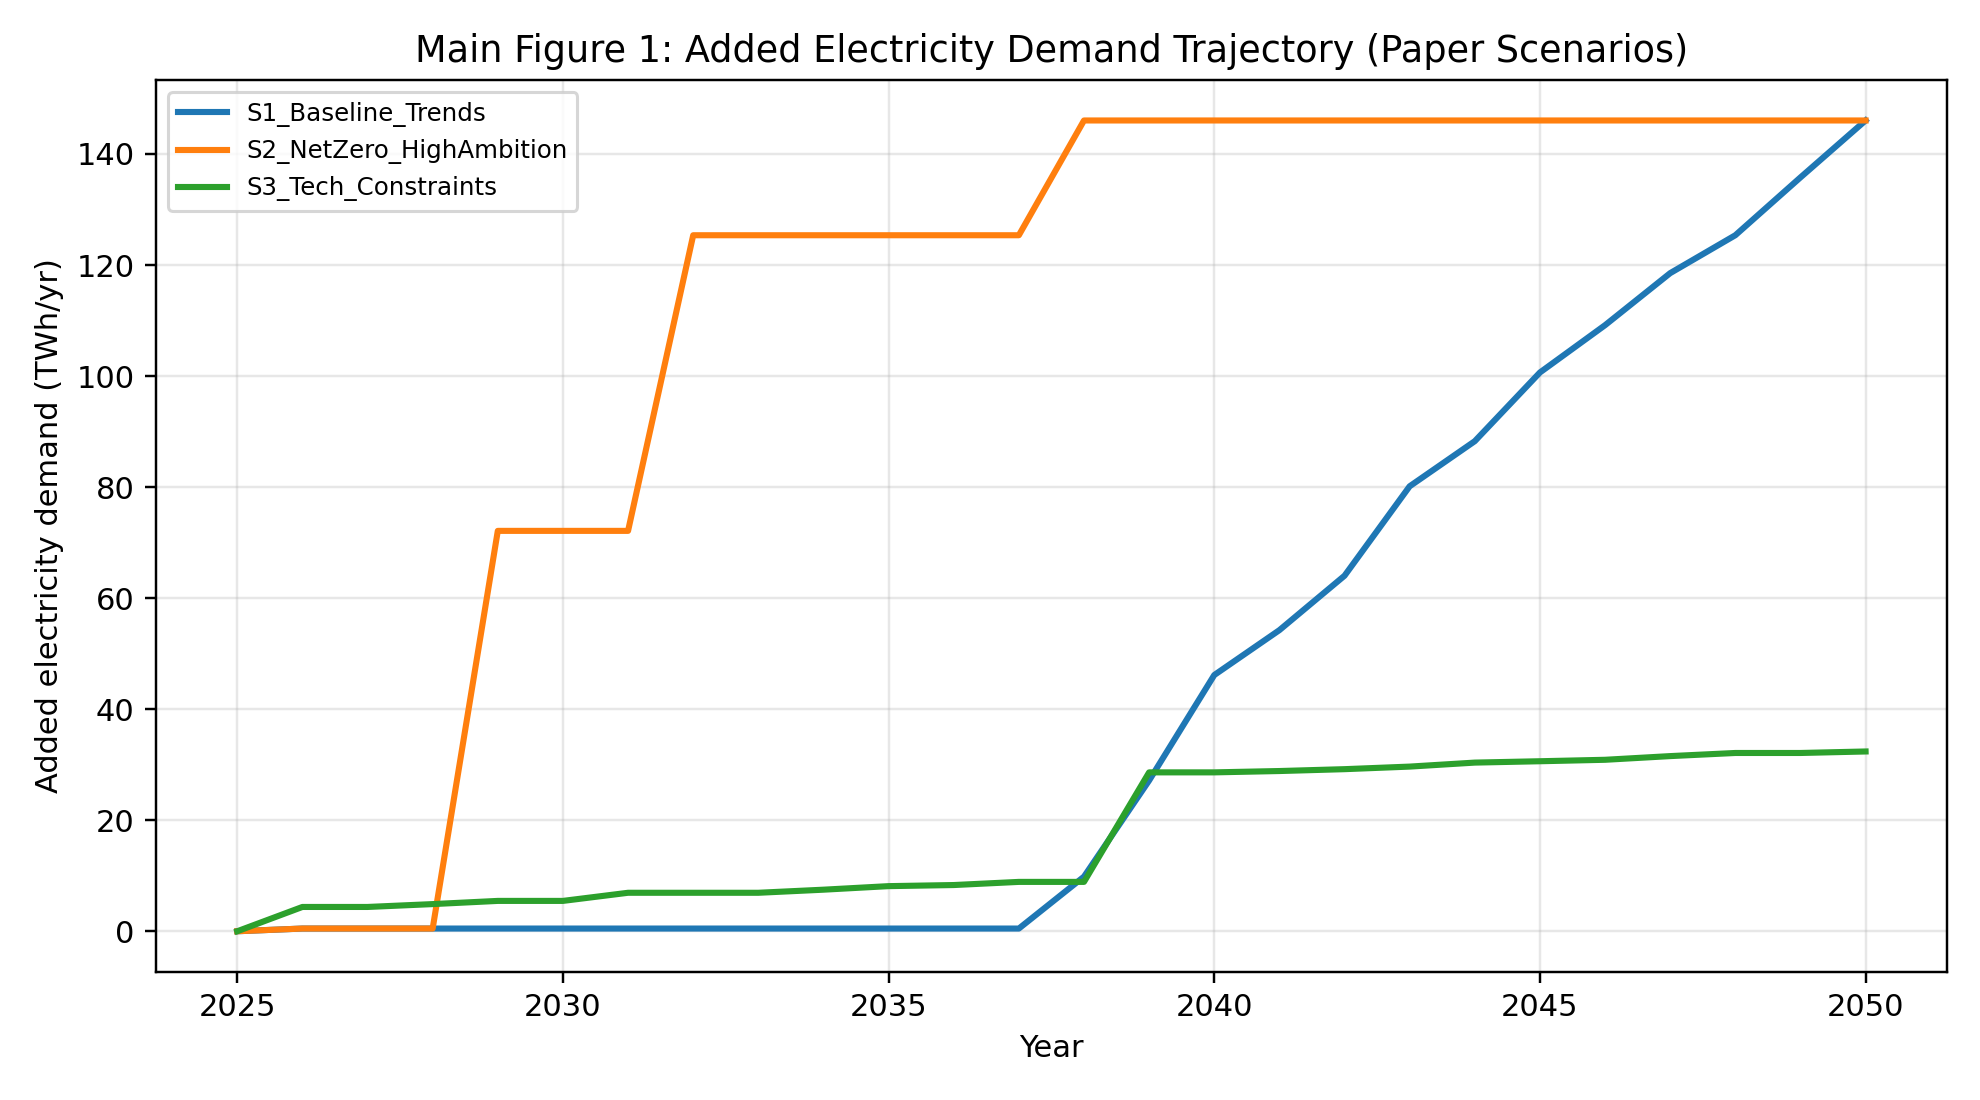
\includegraphics[keepaspectratio,alt={Main Figure 1}]{../02_figures/fig_main_added_electricity_trajectory.png}}
\emph{Added electricity demand trajectory used for infrastructure
bottleneck interpretation.}

\pandocbounded{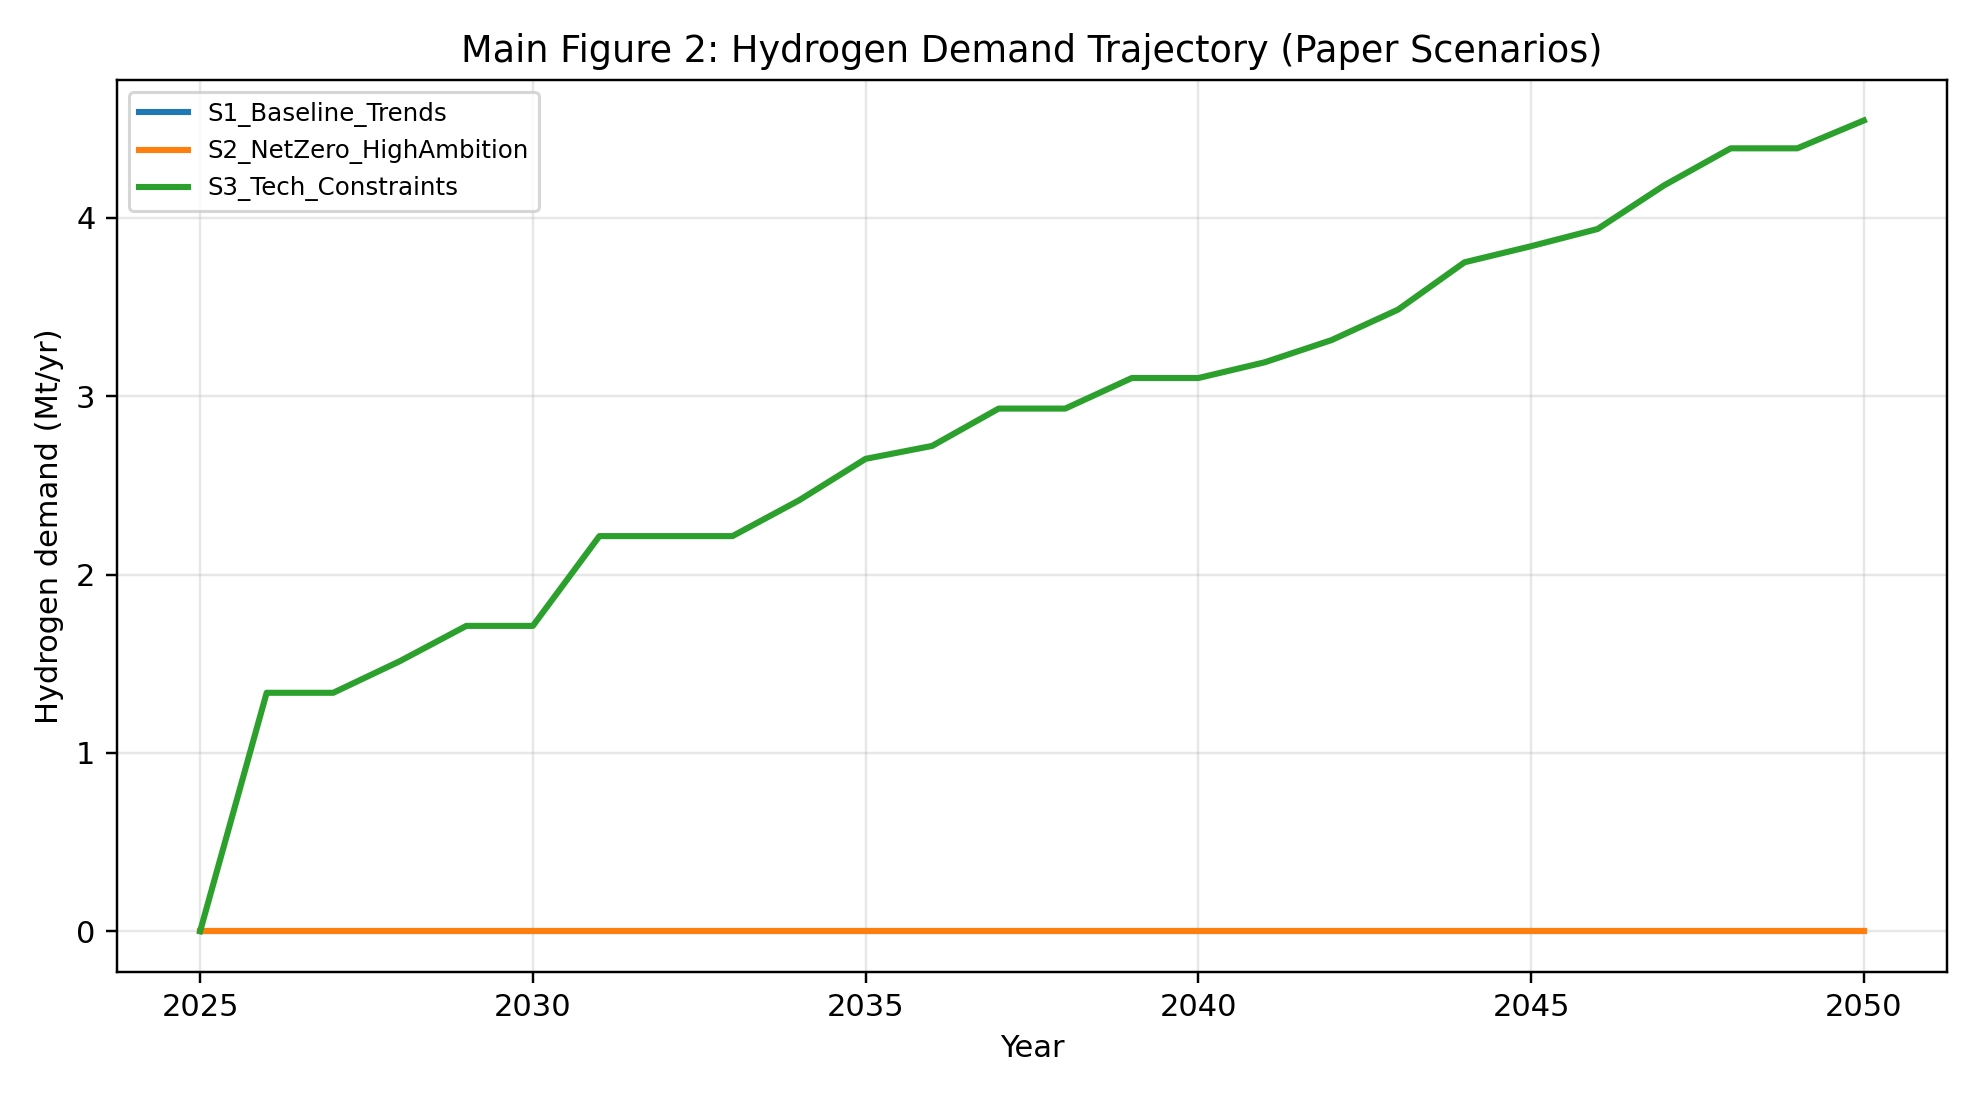
\includegraphics[keepaspectratio,alt={Main Figure 2}]{../02_figures/fig_main_hydrogen_trajectory.png}}
\emph{Hydrogen demand trajectory in paper scenarios.}

\pandocbounded{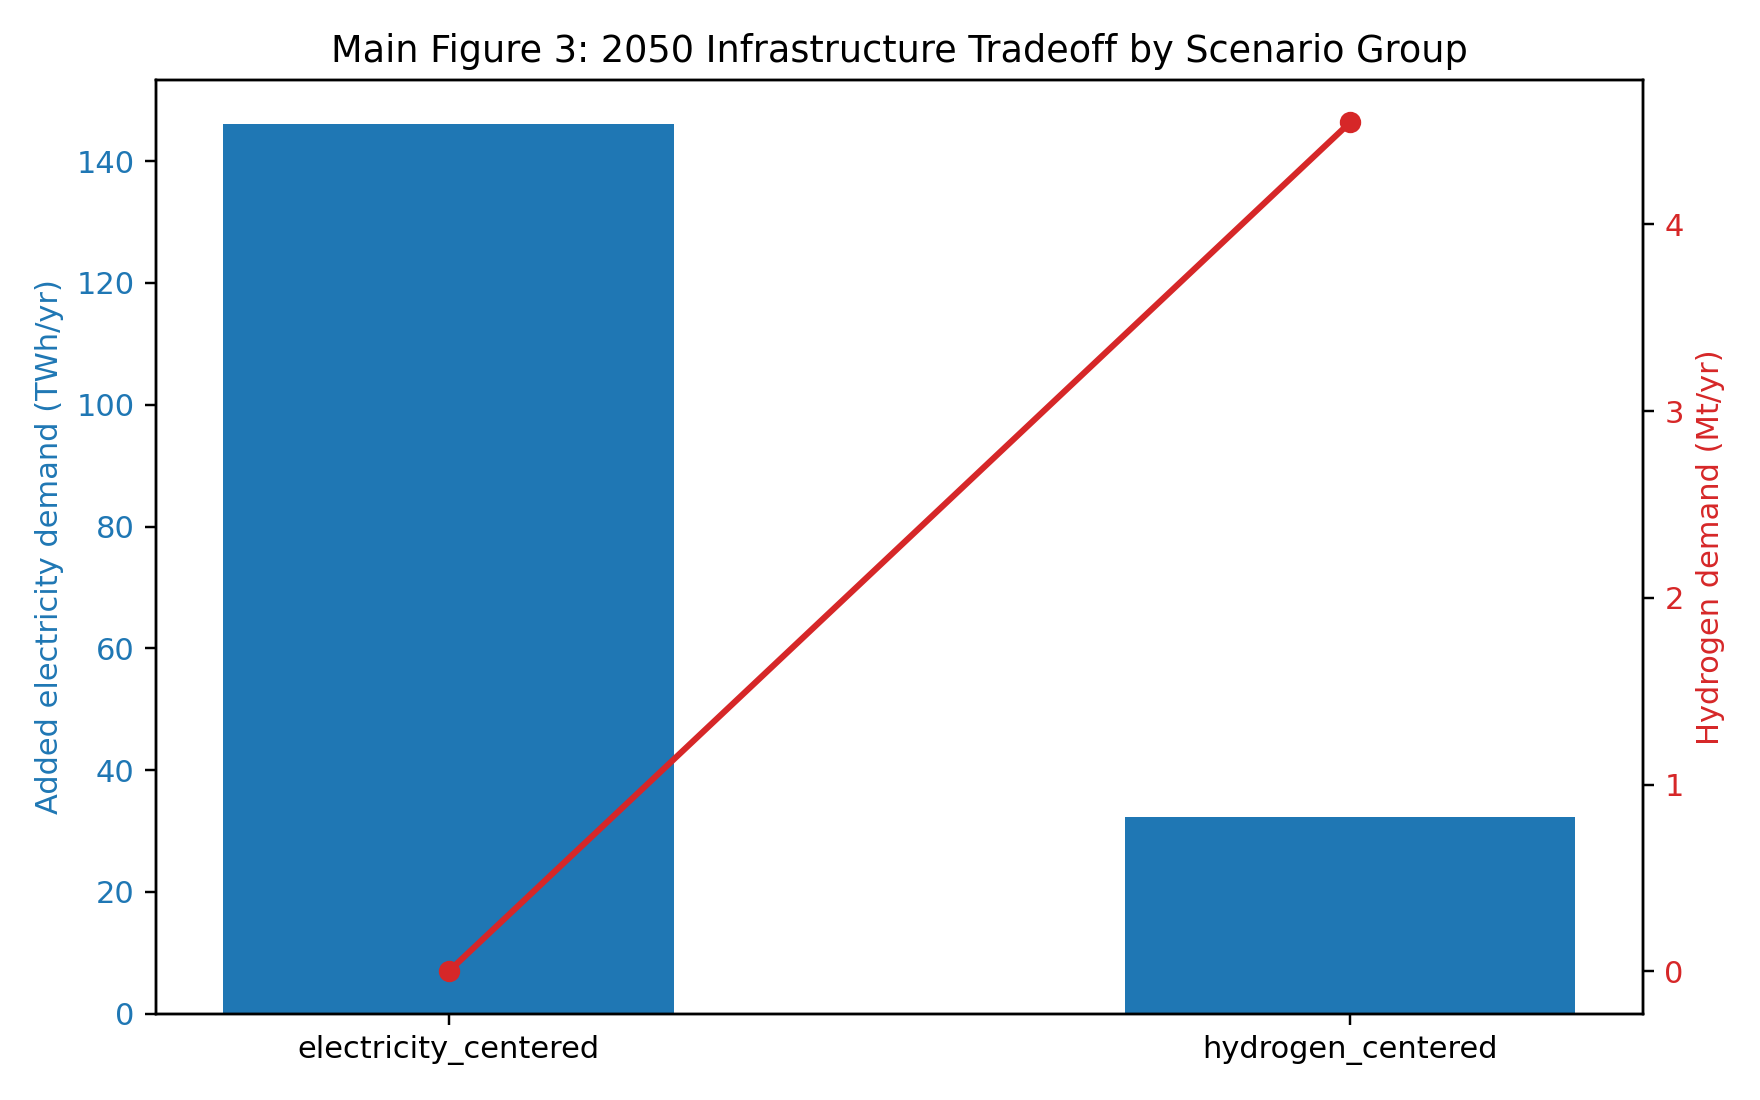
\includegraphics[keepaspectratio,alt={Main Figure 3}]{../02_figures/fig_main_infrastructure_tradeoff_2050.png}}
\emph{2050 infrastructure tradeoff between electricity-centered and
hydrogen-centered scenario groups.}

Main tables are generated in:

\begin{itemize}
\tightlist
\item
  \texttt{../06\_verification/table\_main\_cost\_abatement\_energy\_2030\_2040\_2050.csv}
\item
  \texttt{../06\_verification/table\_main\_infrastructure\_requirements\_2050.csv}
\end{itemize}

Legacy MAC curves are retained as supplementary diagnostics.

\subsection{4. Discussion}\label{4-discussion}

\subsubsection{4.1 Interpretation of H1}\label{41-interpretation-of-h1}

The evidence supports H1: pathway outcomes are materially shaped by
infrastructure requirements. Cost-only ranking does not describe
feasibility when electricity and hydrogen supply constraints are
binding.

\subsubsection{4.2 Policy implications linked to computed
evidence}\label{42-policy-implications-linked-to-computed-evidence}

\begin{itemize}
\tightlist
\item
  Early grid reinforcement must be planned against electricity-centered
  demand growth up to \textbf{146.034 TWh/yr} added demand in 2050.
\item
  Hydrogen strategy must include supply-chain scaling for \textbf{4.546
  Mt/yr} hydrogen by 2050 in hydrogen-centered pathways.
\item
  Mixed portfolios should be assessed through integrated infrastructure
  planning, not separate technology cost screens.
\end{itemize}

\subsubsection{4.3 Limitations
(evidence-only)}\label{43-limitations-evidence-only}

\begin{itemize}
\tightlist
\item
  Scope 3 emissions are outside the optimization boundary.
\item
  The manuscript excludes unexecuted analyses from core claims.
\item
  Results depend on scenario assumptions embedded in the provided
  datasets.
\end{itemize}

\subsection{5. Conclusion}\label{5-conclusion}

This study reframes petrochemical decarbonization from a static
cost-ranking problem to an infrastructure-feasibility problem. The
verified evidence shows that both electrification-led and hydrogen-led
pathways impose large but different infrastructure requirements.
Therefore, transition policy should prioritize sequencing and investment
in grid and hydrogen systems as the primary enablers of credible
net-zero pathways.

\subsection{Administrative
declarations}\label{administrative-declarations}

\begin{itemize}
\tightlist
\item
  \textbf{Funding:} No external funding was received for this study.
\item
  \textbf{Conflict of interest:} The author declares no competing
  interests.
\item
  \textbf{Data availability:} All evidence files used in this manuscript
  are contained in \texttt{../03\_data/} and
  \texttt{../06\_verification/}.
\end{itemize}

\end{document}
